\documentclass{article}
\usepackage{tikz}
\usetikzlibrary{arrows.meta,positioning,backgrounds}
% named styles: the drawing canvas lists them, edits them and applies them by name
\tikzset{box/.style={draw, rounded corners, fill=blue!10}, flow/.style={-Stealth, thick}}
\begin{document}
A pipeline, drawn with styles. Open \emph{Edit drawing} on the picture.

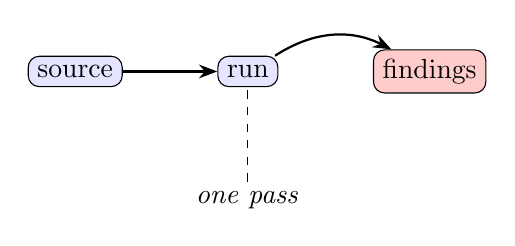
\begin{tikzpicture}[node distance=1.2cm, hot/.style={fill=red!20}]
  \node[box] (src) {source};
  \node[box, right=of src] (run) {run};
  \node[box, hot, right=of run] (out) {findings};
  \node[below=of run] (note) {\emph{one pass}};
  \draw[flow] (src) -- (run);
  \draw[flow] (run) to[bend left=30] (out);
  \draw[dashed] (note) -- (run);
\end{tikzpicture}
\end{document}
